%	To produce Postscript and PDF:
%    latex template; latex template; 
%    dvips -o template.ps template; ps2pdf template.ps
\documentclass[a4paper,11pt]{article}
\usepackage{mathptmx}
%\usepackage{newtxmath}   not available ? 
%\usepackage{newtxtext} []  not available ?
\usepackage[margin=28mm]{geometry}% <-------- CHANGE HERE for the global margins
\usepackage[T1]{fontenc}    % Check that ÖÄÅöäå come out ok!
\usepackage[utf8]{inputenc}
\usepackage{graphicx}
\usepackage{url} 
\usepackage{parskip}
\usepackage{listings} % for code snippets
\usepackage{authblk}
\usepackage[nobottomtitles]{titlesec}
\linespread{1.1}
\usepackage[bottom]{footmisc}
\usepackage[title]{appendix}
\usepackage{perpage} %the perpage package
\MakePerPage{footnote} %the perpage package command
\usepackage{varioref} %for \vref
\usepackage{enumitem}
\usepackage{wrapfig}
\usepackage[table]{xcolor} % for table colors (gray)
\usepackage{caption}
%
% should not USE  ? 
%\setlength{\parindent}{10mm} % Do not indent the 1st line of a paragraph.
%\setlength{\parskip}{20mm}   % Add space between paragraphs.

% defined new environments
\newenvironment{filecode}[1][]
  {\minipage{\linewidth}% \begin{filecode}[#1]
   \lstset{basicstyle=\ttfamily\footnotesize,#1}}
  {\endminipage}% \end{filecode}

\newenvironment{note}[1]
  {
  \vspace{1em}\hspace{1.5em}
  \hbox{%
  \vrule\hspace{.5em}\parbox{.9\textwidth}%
  {
  \textbf{Note:}
  #1
  }}}
  {\vspace{1em}}

\renewenvironment{abstract}
{\itshape \small
  \begin{center}
  \bfseries \abstractname\vspace{-.5em}\vspace{0pt}
  \end{center}
  \list{}{
    \setlength{\leftmargin}{1.5cm}%
    \setlength{\rightmargin}{\leftmargin}%
  }%
  \item\relax}
{\endlist}


% defines my code style
\usepackage{color}
\usepackage{courier}

\definecolor{dkgreen}{rgb}{0,0.6,0}
\definecolor{gray}{rgb}{0.5,0.5,0.5}
\definecolor{mauve}{rgb}{0.58,0,0.82}

\lstset{frame=tb,
  language=Java,
  aboveskip=3mm,
  belowskip=3mm,
  showstringspaces=false,
  columns=flexible,
  basicstyle={\scriptsize\ttfamily},
  numbers=left,
  numbersep=4pt,
  numberstyle=\scriptsize\color{gray},
  keywordstyle=\color{blue},
  commentstyle=\color{dkgreen},
  stringstyle=\color{mauve},
  moredelim=[s][\color{gray}]{@}{\ },
  breaklines=true,
  breakatwhitespace=true,
  tabsize=2
}

\lstdefinelanguage{JavaScript}{
  keywords={typeof, new, true, false, catch, function, return, null, catch, switch, var, if, in, while, do, else, case, break},
  keywordstyle=\color{blue},
  ndkeywords={class, export, boolean, throw, implements, import, this},
  ndkeywordstyle=\color{gray},
  identifierstyle=\color{black},
  sensitive=false,
  comment=[l]{//},
  morecomment=[s]{/*}{*/},
  commentstyle=\color{dkgreen}\ttfamily,
  stringstyle=\color{blue}\ttfamily,
  morestring=[b]',
  morestring=[b]"
} 

% title variable definition
\newcommand{\mahtitle}{Fuzzy logic in Neural networks}

% Save some paper by stuffing more text on each page:
% A4: 210mm x 297mm, approximately 35 mm margins on every side.
\addtolength{\topmargin}{-2mm}    
\addtolength{\textheight}{2mm}    
%\addtolength{\oddsidemargin}{-10mm} 
%\addtolength{\textwidth}{14mm}     

% This creates the header.
\makeatletter
\renewcommand{\@oddhead}
{\fontsize{10}{12}\selectfont \hfill \mahtitle \hfill }
\makeatother

\renewcommand{\Authfont}{\Large\normalfont}
\renewcommand{\Affilfont}{\large\itshape}

\begin{document}

%============================================================
% title
\label{Title} 
\title{\mahtitle \vspace{1pc}}
\author{Patryk Małek \vspace{-0.7pc}}
\affil{
        University of Novi Sad\\
        Faculty of Sciences\\
        malekpatryk@gmail.com
      }
\date{}%\date{\today}         % Do not print the date on the final paper!
\maketitle
% prevents page numbering on this page
\thispagestyle{empty}

%============================================================

\vspace{5pc}
\centerline{

\includegraphics[width=0.35\textwidth,height=0.35\textheight,keepaspectratio]{NoviSadLogoGray.jpg}
}
\vspace{11pc}

\begin{abstract}
\label{Abstract}
Initially a theory, nowadays fuzzy logic has become an operational technique.
Used alongside other advanced techniques, it is making a discrete but appreciated appearance in many fields of computer science.
Together with Artificial Neural Networks they are able to create powerful systems when used properly.
This paper intends to present basics of fuzzy logic and aritficial neural networks in theory and will try to present some trivial practical usage of both of those techniques.
\end{abstract}

%============================================================

%\tableofcontents

%============================================================

\pagebreak
\section{Introduction} 
\subsection{Background}
Both neural networks and fuzzy systems have some things in common. They can be used for solving a problem (e.g. pattern recognition, regression or density estimation) if there does not exist any mathematical model of the given problem. They solely do have certain disadvantages and advantages which almost completely disappear by combining both concepts.

Neural networks can only come into play if the problem is expressed by a sufficient amount of observed examples. These observations are used to train the black box. On the one hand no prior knowledge about the problem needs to be given. On the other hand, however, it is not straightforward to extract comprehensible rules from the neural network's structure.

On the contrary, a fuzzy system demands linguistic rules instead of learning examples as prior knowledge. Furthermore the input and output variables have to be described linguistically. If the knowledge is incomplete, wrong or contradictory, then the fuzzy system must be tuned. Since there is not any formal approach for it, the tuning is performed in a heuristic way. This is usually very time consuming and error-prone.

\begin{table}[h]
\centering
    \begin{tabular}{ | l | l | }
	    \hline
	    \rowcolor{gray!20}
		\multicolumn{1}{|c|}{\textbf{Neural Networks}} & \multicolumn{1}{|c|}{\textbf{Fuzzy Systems}} \\ \hline % multicolumn makes it center with |c|
		%\textbf{Neural Networks} & \textbf{Fuzzy systems}\\ \hline
	    no mathematical model necessary & no mathematical model necessary\\ \hline
	    learning from scratch & apriori knowledge necessary \\ \hline
	    several learning algorithm & not capable to learn \\ \hline
	    black box behavior & simple interpretation and implementation \\ \hline
    \end{tabular}
    \caption{Comparison of neural networks and fuzzy systems}
    \label{tab:comparison_neur_ann}
\end{table}

As shown in the table ~\ref{tab:comparison_neur_ann} we can see that fuzzy systems and neural networks have quite contrary traits which connected can create a very powerful system.

\subsection{Fuzzy logic}
There are many misconceptions about fuzzy logic.
Fuzzy logic is not fuzzy.
Basically, fuzzy logic is a precise logic of imprecision and approximate reasoning.

In real world, we do not assign precise parameters or criteria to most objects that we encounter on every day basis.
For instance we would not describe a rock lying on a side of the road being 4.23m in diameter.
Normally we would call it just big or huge or some other \emph{linguistic expression} that we would find suitable.
That is something that we people use in our everyday lives and do now acknowledge it.
Computers have hard time describing 
Although fuzzy logic has been studied since 1920s (as study of infinite-valued logic), the term ``fuzzy sets'' has been coined by Lofti A. Zadeh, a professor at the University of California at Berkley in his article ``Fuzzy sets'' in 1965 \cite{fuzzy_sets_zadeh} as a mean to model the uncertainty
of natural language.
He was trying to argument for his idea saying that people do not require precise, numerical information input, and yet they are capable of highly adaptive control and if one had been able to program a system to accept noisy, imprecise input it would have been much more effective than contemporary systems.

Fuzzy systems:
\begin{itemize}
\item Are inherently robust since they do not require precise, noise-free inputs and can be programmed to fail safely if a feedback sensor quits or is destroyed. The output control is a smooth control function despite a wide range of input variations,
\item Are not limited to few feedback inputs and one or two outputs, nor is it necessary to measure or compute rate-of-change parameters in order for it to be implemented. Any control data that provides some indication of system's actions and reactions is sufficient. This allows the fuzzy systems to be inexpensive and imprecise thus keeping the overall system cost and complexity low,
\item Since fuzzy logic controller processes user-defined rules governing the target control system, it can be modified and tweaked easily to improve or drastically alter system performance. New sensors can easily be incorporated into the system simply by generating appropriate governing rules,
\item Because of the rule-based operation, any reasonable number of inputs can be processed and numerous outputs generated, although defining the rulebase quickly becomes complex if too many inputs and outputs are chosen for a single implementation since rules defining their interrelations must also be defined. It would be better to break the system into smaller chunks and use several smaller fuzzy controllers distributed on the system, each with more limited responsibilities,
\item Fuzzy systems can control nonlinear systems that would be difficult or impossible to model mathematically. This opens doors for control systems that would normally be deemed unfeasible for automation.
\end{itemize}

\subsection{Artificial Neural Networks}
Having nowadays ``traditional'' computer systems we can use it efficiently to some extent in various scenarios and for various purposes, e.g. multimedia systems, video games, document editing, algebra or arithemics.

\begin{table}[h]
\centering
    \begin{tabular}{ | l | l | }
	    \hline
	    \rowcolor{gray!20}
		\multicolumn{2}{|c|}{\textbf{Everyday computer systems}} \\ \hline % multicolumn makes it center with |c|
	    \rowcolor{gray!35}
		\multicolumn{1}{|c|}{\textbf{Good at}} & \multicolumn{1}{|c|}{\textbf{Not so good at}} \\ \hline % multicolumn makes it center with |c|
	    fast arithmetic & massive parallelism \\ \hline
	    precisely executing programmed commands & working with noisy inputs \\ \hline
	    \multicolumn{1}{|c|}{-} & adapting to tolerances \\ \hline
	    \multicolumn{1}{|c|}{-} & adapting to changing curcumstances\\ \hline
    \end{tabular}
    \caption{Traits of everyday, traditional computer systems.}
    \label{tab:everyday_computer_systems}
\end{table}Artificial neural networks are computational models inspired by human's brain, that are capable of machine learning and pattern recognition.

When some more abstract human like processing comes to play like defining a structure/model based on a concrete data set, prediction based on an example set then traditional computers start to pant.
That's were artificial neural networks come to place.


Artificial neural networks are usually presented as systems of interconnected ``neurons'' (just like human brain's neurons, hence the name), that can compute values from inputs by feeding information through the network.


\begin{wrapfigure}{r}{0.45\textwidth}
	\vspace*{-2em}
	\hspace*{1em}
	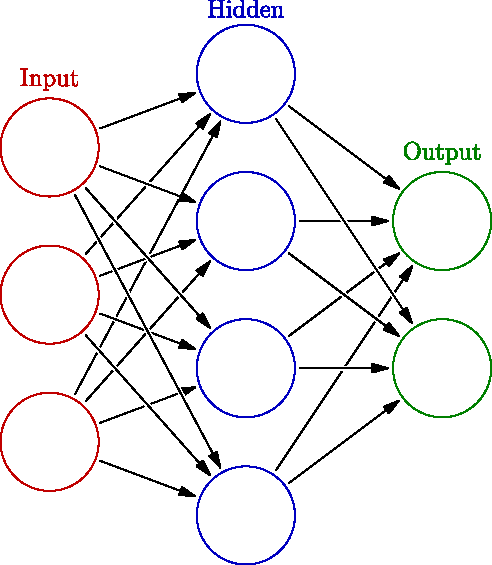
\includegraphics[width=0.43\textwidth]{images/ann_wiki_model.pdf}
	%[height=0.4\textheight,keepaspectratio]
	\caption{Artificial neural network model showing its free layers: inputs, hidden layer and output layer.~\cite{wiki_ann}}
	\label{fig:ann_model}
\end{wrapfigure}

They use learning algorithms that are inspired by understanding of how the brain learns, but they are evaluated by how well they work for practical applications such as speech recognition, object recognition, image retrieval and the ability to recommend products that a user will like.
Despite being quite powerful when properly designed artificial neural networs are orders of magnitude less complex than human brains.
As computers become more powerful, artificial neural networks are gradually taking over from simpler machine learning methods.
They are already at the heart of a new generation of speech recognition devices and they are beginning to outperform earlier systems for recognizing objects in images.

\vspace*{5em}





%============================================================

\section{Fuzzy neural networks}
The term fuzzy neural network (neuro-fuzzy) refers to combinations of artificial neural networks and fuzzy logic.
Neurofuzzy hybridization results in a hybrid intelligent system that connects these two techniques by combining the human-like reasoning style of fuzzy systems with learning and connectionist structure of neural networks.
Human-like reasoning style of fuzzy systems is incorporated to FNNs through the use of fuzzy sets and a linguistic model consisting of a set of IF-THEN fuzzy rules.
The main strength of neurofuzzy systems is that they are universal approximators with the ability to solicit interpretable IF-THEN rules.

\subsection{Fuzzy neurons}
Fuzzy neurons are neurons that follows the basic idea of artificial neurons with small changes:

\begin{itemize}
\item The inputs to the fuzzy neurons $x_1, x_2, \dots, x_n$ represent fuzzy labels of fuzzy input variables,
\item The weights $w_i$ are replaced by functions $\mu_i$ which are the membership functions of the fuzzy labels $x_i \in (i = 1, 2, \dots, n)$,
\item Excitatory connections are represented by MIN operation and inhibitory connections by fuzzy logic complements followed by MIN operation,
\item Threshold level is not assigned.
\end{itemize}

In those fuzzy neurons learning is not present.
Membership functions attached to neuron connections are not changing.

\clearpage
To improve those traits of fuzzy neuron, Yamakwa et al. in 1992~\cite{yamakawa} came up with the idea of \emph{neo-fuzzy neurons} as a follow up to fuzzy neurons.
Those neurons differ to previously described fuzzy neurons in:

\begin{itemize}
\item Their inputs $x_1, x_2, \dots, x_n$ represent fuzzy variables,
\item In addition to the membership function $\mu_{ij}$ , which is bound to the input segment $x_{ij}$, weights $w_ij$ are also assigned, subject to a training procedure,
\item The segments $x_{i1}, x_{i2}, \dots, x_{il}$ have standard triangular membership functions; thus an input activates only two membership functions simultaneously; the sum of the degree to which an input value x'i belongs to any two neighboring membership functions $\mu_{ik}(x_i')$ and $\mu_{i,k+1}(x_i')$ is always equal to 1.
\end{itemize}

The model of neo-fuzzy neuron together with detailed diagram of its nodes and membership functions attached to its connection is depicted in Figure~\ref{fig:neuro_fuzzy_model}.

\begin{figure}[h!]
  \centering
	\captionsetup{width=24pc}
    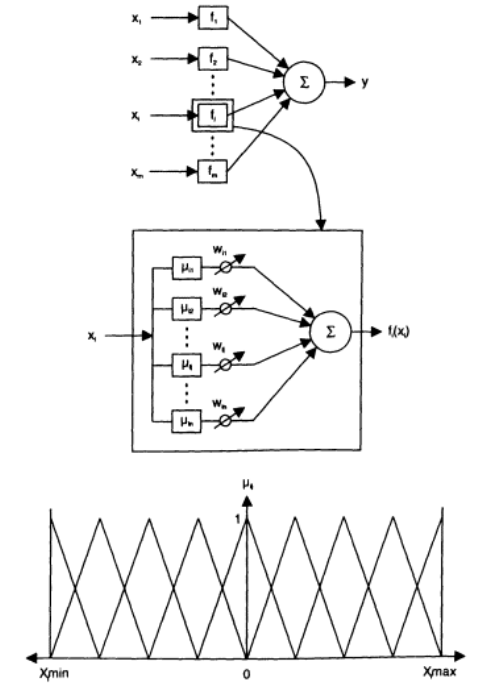
\includegraphics[width=0.55\textwidth]{images/neuro_fuzzy_model.png}
	\caption{Yamakawa's neo-fuzzy neuron. Each of the $m$ functions $f_i, i \in (1, 2, ..., m)$ bound to each of the $m$ inputs $x_i$ are represented by n = 9 fuzzy membership functions $T_ij$ , standard triangular ones uniformly distributed over the universe $Ux_i$ , as well as by corresponding weights $w_{ij}$ which are subject to change during training.}
	\label{fig:neuro_fuzzy_model}
\end{figure}

\subsection{Fuzzy neural networks}
Similar to the way the fuzzy neuron and the neo-fuzzy neuron were created, different types of fuzzy neural networks (FNNs) have been developed and applied to different tasks.
A fuzzy neural network is a connectionist model for fuzzy rules implementation and inference. There is a great variety of architectures and functionalities of FNN.
The FNNs developed so far differ mainly in the following parameters:
\begin{itemize}
\item Type of fuzzy rules implemented; this affects the connection structure used,
\item Type of inference method implemented; this affects the selection of different neural network parameters and neuronal functions, such as summation, activation, and output function. It also influences the way the connection weights are initialized before training, and interpreted after training,
\item Mode of operation: we consider here three major modes of operation by:
	\begin{enumerate}
	\item Fixed mode, fixed membership functions-fixed set of rules, that is, a fixed set of rules is inserted in a network, the network performs inference, but does not change its weights,
	\item Learning mode, that is, a neural network is structurally defined to capture knowledge in a certain format, for example, some type of fuzzy rules. The network architecture is randomly initialized and trained with a set of data. Rules are then extracted from the structured network. The rules can be interpreted either in the same network structure or by using other inference methods.
	\item Adaptation mode. A neural network is structurally set according to a set of existing rules, ``hints,'' heuristics. The network is then trained with new data and updated rules are extracted from its structure.
	\end{enumerate}
\end{itemize}

Two cases can be distinguished here: (1) fixed membership functions—adaptable rules and (2)
adaptable membership functions—adaptable rules.
To summarize the above, FNNs have two major aspects:
\begin{enumerate}
\item Structural. A set of rules is used to define the initial structure of a neural network; two types of neural networks have been mainly used so far: (a) multilayer perceptrons (MLPs), and (b) radial-basisfunctions networks.
\item Functional, parametric. After having defined the structure of a neural network and possibly having trained it with data, some parameters can be observed that would explain the inference which the network performs. Those parameters can be used to derive a (fuzzy) rule-based system represented in linguistic terms.
\end{enumerate}


%============================================================

\clearpage
\section{Summary} 

As of \cite{fuzzy_db} and \cite{seattlerobotics} and \cite{fuzzy_sets_zadeh}

%============================================================

\clearpage
\label{Bibliography} 
%
\bibliographystyle{siam}
\footnotesize{ \bibliography{bibliography} }
% In that case, remember to run bibtex:
% latex template; bibtex template; latex template; latex template; 

%============================================================

%\clearpage
%\begin{appendices}
%
%\section{Extending GLSurfaceView class to capture user input.}
%\label{App:Appendix_A}
%\begin{filecode}[label=lst:glsurfaceview_override]
%\lstinputlisting{./code/opengles_glsurfaceview_override.java}
%\end{filecode}
%
%\end{appendices}

\end{document}